\documentclass[a4paper,10pt]{article}
%\usepackage[active]{srcltx}

\usepackage{amsmath}
\usepackage{amsfonts}
\usepackage{amssymb}
\usepackage{amsthm}
\usepackage[utf8]{inputenc}
\usepackage[czech]{babel}
\usepackage{graphicx}

%
\def\div{{\rm div}}
\def\Lapl{\Delta}
\def\grad{\nabla}
\def\supp{{\rm supp}}
\def\dist{{\rm dist}}
%\def\chset{\mathbbm{1}}
\def\chset{1}
%
\def\Tr{{\rm Tr}}
\def\to{\rightarrow}
\def\weakto{\rightharpoonup}
\def\imbed{\hookrightarrow}
\def\cimbed{\subset\subset}
\def\range{{\mathcal R}}
\def\leprox{\lesssim}
\def\argdot{{\hspace{0.18em}\cdot\hspace{0.18em}}}
\def\Distr{{\mathcal D}}
\def\calK{{\mathcal K}}
\def\FromTo{|\rightarrow}
\def\convol{\star}
\def\impl{\Rightarrow}
\DeclareMathOperator*{\esslim}{esslim}
\DeclareMathOperator*{\esssup}{ess\,supp}
\DeclareMathOperator{\ess}{ess}
\DeclareMathOperator{\osc}{osc}
\DeclareMathOperator{\curl}{curl}
%
%\def\Ess{{\rm ess}}
%\def\Exp{{\rm exp}}
%\def\Implies{\Longrightarrow}
%\def\Equiv{\Longleftrightarrow}
% ****************************************** GENERAL MATH NOTATION
\def\Real{{\rm\bf R}}
\def\Rd{{{\rm\bf R}^{\rm 3}}}
\def\RN{{{\rm\bf R}^N}}
\def\D{{\mathbb D}}
\def\Nnum{{\mathbb N}}
\def\Measures{{\mathcal M}}
\def\d{\,{\rm d}}               % differential
\def\dx{\d x}
\def\sdodt{\genfrac{}{}{}{1}{\rm d}{{\rm d}t}}
\def\dodt{\genfrac{}{}{}{}{\rm d}{{\rm d}t}}
%
\def\vc#1{\mathbf{\boldsymbol{#1}}}     % vector
\def\tn#1{{\mathbb{#1}}}    % tensor
\def\abs#1{\lvert#1\rvert}
\def\Abs#1{\bigl\lvert#1\bigr\rvert}
\def\bigabs#1{\bigl\lvert#1\bigr\rvert}
\def\Bigabs#1{\Big\lvert#1\Big\rvert}
\def\ABS#1{\left\lvert#1\right\rvert}
\def\norm#1{\bigl\Vert#1\bigr\Vert} %norm
\def\close#1{\overline{#1}}
\def\inter#1{#1^\circ}
\def\eqdef{\mathrel{\mathop:}=}     % defining equivalence
\def\where{\,|\,}                    % "where" separator in set's defs
\def\timeD#1{\dot{\overline{{#1}}}}
%\def\dfrac#1#2{{\textsize\frac{#1}{#2}}}
%
% ******************************************* USEFULL MACROS
\def\RomanEnum{\renewcommand{\labelenumi}{\rm (\roman{enumi})}}   % enumerate by roman numbers
\def\rf#1{(\ref{#1})}                                             % ref. shortcut
\def\prtl{\partial}                                        % partial deriv.
\def\Names#1{{\scshape #1}}
\def\rem#1{{\parskip=0cm\par!! {\sl\small #1} !!}}
%
%
% ******************************************* DOCUMENT NOTATIONS
% document specific
%***************************************************************************
%
\addtolength{\textwidth}{2cm}
\addtolength{\vsize}{2cm}
\addtolength{\topmargin}{-1cm}
\addtolength{\hoffset}{-1cm}
\begin{document}
\parskip=2ex
\parindent=0pt

\section{Iterační metody řešení nelineárních rovnic}
Pokročilejší - realističtější fyzikalní, ekonomické, statistické modely vedou na nelineární rovnice a jejich soustavy.
\subsection{příklady}
\begin{enumerate}
 \item Na kruhovém trávníku o poloměru $1$ se pase koza přivázaná na provaze délky $r$ ke kolíku zatlučenému na okraji trávníku.
 Pro jaké $r$ sežere koza právě polovinu plochy trávníku?

 Vypasená plocha je součet ploch dvou kruhových úsečí, jejichž obsah se spočítá jako rozdíl obsahu příslušné kruhové výseče a
 rovnoramenného trojúhelníku mezi středem a tětivou. Plocha tedy je
\[
 P=\alpha-\frac12 2\sin\alpha\cos\alpha+r^2\beta-\frac12r^22\sin\beta\cos\beta.
\]
 přičemž $\alpha$ a $\beta$ jsou poloviny středových úhlů úsečí a platí pro ně
\[
 \frac{r}{2}=\sin\frac{\alpha}{2},\quad \beta=\frac{\pi}{2}-\frac{\alpha}{2}.
\]
 Plocha $P$ být polovina plochy trávníku, tedy $P=\frac{pi}{2}$. Po dosazení a úpravách pomocí základních trigonometrických vzorců
dostaneme pro $\alpha$ rovnici
\[
 \sin\alpha+(\pi-\alpha)\cos\alpha=\frac{\pi}{2}.
\]

 \item Nalezněte maximum funkce $f(x)=x\sin x$ na intervalu $I=(0,\pi)$.

 Vykreslením grafu funkce snadno zjistíme, že na intervalu $I$ má právě jeden extrém, takže
 bod maxima splňuje rovnici
 \[
    f'(x)=\sin x +x\cos x =0.
 \]
 Která má patrně právě (graf) jeden kořen na $I$.
 \item 


\end{enumerate}



\section{Metoda sítí pro řešení PDR}
Rovnici pro neznámou funkci $u(x_1,x_2,\dots)$, která obsahuje parciální derivace podle proměnných 
$x_1,x_2,\dots$ nazýváme {\it parciální diferenciální rovnicí} (PDR). {\it Řád rovnice} je dán řádem nejvyšší parciální derivace.
Například rovnice
\[
 \frac{\prtl }{\prtl x}\frac{\prtl}{\prtl x} u + \big(\frac{\prtl u}{\prtl y}\big)^3=0
\]
je rovnice druhého řádu pro funkci $u(x,y)$, jelikož nejvyšší derivace v prvním členu je druhého řádu.
Rovnici nazýváme {\it lineární} pokud jsou všechny její členy lineární vzhledem k hledané funkci
respektive jejím derivacím. Uvedená rovnice není lineární, lineární je jen její první člen.
Pokud je lineární alespoň člen nejvyššího řádu nazývá se rovnice {\it kvazilineární}.
 
Základními typy lineárních PDR jsou eliptické, parabolické a hyperbolické rovnice. V dalším se omezíme na
tyto typy rovnic a navíc jen na rovnice druhého řádu. Tyto lineární rovnice jsou základem jednoduchých modelů 
pro množství fyzikálních systémů. Dále je pro tyto rovnice známa obecná
 matematická teorie, která zajišťuje existenci a jednoznačnost řešení a jsou k dispozici 
též spolehlivé numerické metody 
pro jejich řešení. I v případě, že máme pro daný problém k dispozici  přesnější 
nelineárním model a nějakou numerickou metodu pro jeho řešení, je většinou třeba použít linearizovaný model 
pro ověření správnosti příslušného programu. Navíc řešení nelineárních úloh většinou vychází z metod pro lineární 
úlohy.

\subsection{Eliptické rovnice}
Budeme uvažovat jeden z typů eliptických rovnic a to rovnici, která má na $m$-rozměrném prostoru
$\Real^m$ tvar
\begin{equation}\label{ElipRce}
   L u=-\sum_{i,j=1}^m \frac{\prtl}{\prtl x_i}\Big(a_{ij}(\vc x) \frac{\prtl u}{\prtl x_j}\Big) + qu =f.
\end{equation}
Ve vektorovém zápisu lze totéž zapsat
\[
  Lu =- \div ( \tn A(\vc x) \grad u) + qu=f,
\]
kde pro každý bod $\vc x$ je $A(\vc x)$ reálná symetrická ($a_{ij}=a_{ji}$) matice $m\times m$.
Na levé straně rovnice \eqref{ElipRce} jsme zavedli diferenciální operátor $L$ druhého řádu.
Operátor $L$ se nazývá {\it eliptickým} pokud platí
\[
   \sum_{i,j=1}^m a_{ij}(\vc x)\xi_i\xi_j\ge p_0\sum_{i=1}^m \xi_i^2,
\]
tedy pokud je matice $\tn A(\vc x)$ stejnoměrně pozitivně definitní pro všechny body $\vc x$.
Speciálním případem operátoru $L$ pro $\tn A=\tn E$ a $q=0$ je {\it Laplaceův operátor}
\[
   \Lapl u=\sum_{i=1}^m \frac{\prtl^2 u}{\prtl x_i^2}=\div\grad u.
\]

Rovnici \eqref{ElipRce} většinou neuvažujeme na celém prostoru, ale na nějaké omezené oblasti
$\Omega\subset\Real^m$.
Z teorie vyplývá, že pro jednoznačnost řešení je třeba doplnit rovnici okrajovými
podminkami na hranici $\Gamma=\prtl\Omega$ oblasti $\Omega$. Okrajová podmínka má obecně tvar
\begin{equation}\label{BC}
   \alpha(\vc x)\sum_{i,j=1}^m a_{i,j}(\vc x) \frac{\prtl u}{\prtl x_i} n_j+\beta(\vc x) u\equiv
   \alpha(\vc x)\vc n \tn A(\vc x) \grad u +\beta(\vc x) u =\phi(\vc x).
\end{equation}
Pokud je na hranici zadána hodnota hledané funkce $u$  (tj. $\alpha(\vc x) =0$) mluvíme o {\it Dirichletově okrajové podmínce} pokud je zádána derivace (tj. $\beta(\vc x)=0$) jedná se o {\it Neumanovu podmínku}. Obecná smíšená podmínka
\eqref{BC} se nazývá {\it Newtonova okrajová podmínka}.

Nutnost zadat okrajouvou podmínku na celé hranici $\Gamma$ můžeme demonstrovat na jednorozměrném případě,
kdy rovnice \eqref{ElipRce} je obyčejnou diferenciální rovnicí. Prostor řešení takové rovnice má dimenzi $2$. 
Pro obdržení jednoznačného řešení, je tedy potřeba zadat dvě okrajové podmínky na obou koncích oblasti/intervalu $\Omega$. Na jedno rozměrném příkladě si ukážeme ještě záludnost Neumanových podmínek.
Pokud jsou v krajních bodech intervalu zadány pouze derivace $u$ a pokud je 
v rovnici $q=0$, bude rovnice i okrajová podmínka splněna i pro libovolnou funkci $u+C$, kde $C$ je libovolná konstanta.
Tady v tomto případě opět nedostáváme jednoznačnost a je potřeba řešení nějak zafixovat v závislosti na fyzikálním kontextu. Stejně tak pokud je rovnice \eqref{ElipRce} doplněna pouze Neumanovou okrajovou podmínkou, je řešení jednoznačné až na aditivní konstantu. Na druhou stranu data okrajové podmínky, funkci $\phi$, a pravou stranu rovnice $f$ nemůžeme volit libovolně.
Pokud totiž vyintegrujeme rovnici \eqref{ElipRce} přes oblast $\Omega$ a použijeme Greenovu větu pro integrování per-partes v divergenci, dostaneme podmínku
\[
  \int_\Omega f- qu\dx=\int_\Omega L u \dx=\int_\Gamma \vc n\tn A(\vc x) \grad u\d\sigma=
  \int_\Gamma \phi\d\sigma,
\]
která svazuje data okrajové podmínky $\phi$ s pravou stranou $f$.
Pokud je rovnice správným modelem fyzikální skutečnosti, měla by být tato podmínka splněna. Ovšem
při numerickém řešení by bylo potřeba najít diskrétní analogii této podmínky a zajistit, ze jí vstupní data splňují.



Eliptické rovnice tvaru \eqref{ElipRce} modelují množství fyzikálních problémů jako
různé typy difúze, šíření kapaliny v porézním prostředí, zjednodušené modely proudění tekutin, atd. 
Jako typický příklad popíšeme podrobněji problém rozložení teploty v tělese např. chladiči. 
Oblast $\Omega$ reprezentuje chladič, matice $A(\vc x)=p(\vc x)I$ resp. funkce $p$ udává 
proměnnou tepelnou vodivost v objemu chladiče. Dirichletova okrajová podmínka představuje kontakt chladiče 
s rezervoárem s konstantní teplotou (chladící médium) a Neumanova podmínka modeluje plošný zdroj tepla s 
konstantním tepelným tokem (např. procesor). Ve specifických úlohách bychom mohli uvažovat nenulovou pravou 
stranu $f$, která v tomto případě modeluje objemové zdroje tepla, které by mohli být způsobeny např. 
radioaktivitou, nebo chemickými ději v chladiči. Hledaná funkce $u$ je pak rozložení teploty v chladiči. 
V praxi by nás zajímaly zejména teploty v blízkosti Neumanovy okrajové podmínky, abychom zjistili, na 
jakou teplotu jsme schopni chladit zdroj tepla.


\subsection{Metoda sítí pro eliptické rovnice}
V dalším se omezíme na dvourozměrný prostor tedy $m=2$, $\Omega$ je rovinná oblast a její hranice $\Gamma$ je 
uzavřená křivka.
Dále budeme předpokládat eliptický operátor $L$ s maticí tvaru $A(\vc x)=p(\vc x)\tn E$, kde $p$ je daná skalární funkce
prostorové proměnné.
Oblast $\Omega$ pokryjeme sítí bodů a hledanou funkci $u$ budeme přibližně reprezentovat jen 
hodnotami v těchto bodech. Konkrétně budeme předpokládat pravidelnou čtvercovou síť s krokem $h$.
Pro pevné $h$ je uvnitř omezené oblasti $\Omega$ konečné množství bodů $x_i$, $i=1,\dots, N$.
Neznámými jsou funkční hodnoty $u_i$ přibližného řešení. Pro jejich určení je třeba aproximovat
vhodným způsobem derivace v rovnici \eqref{ElipRce} a okrajové podmínce \eqref{BC} a v každém bodě
$x_i$ sestavit aproximativní rovnici. Dostaneme tak soustavu $N$ rovnic jejímž řešením získáme přibližné hodnoty $u_i$ hledané funkce $u$ v bodech $x_i$.

Diferenciální operátor $L$ aproximujeme diferenčním operátorem $L_h$ definovaným v bodě $(x,y)$ takto
\begin{align}\label{AproxL}
  (L_h u)(x,y)&=\frac1{h^2}\Big[\big(p(x+\tfrac h2,y)+p(x-\tfrac h2,y)+p(x,y+\tfrac h2)+p(x,y-\tfrac h2)\big) u(x,y)\\
\notag        &-p(x+\tfrac h2,y)u(x+h,y)-p(x-\tfrac h2,y)u(x-h,y)\\
\notag        &-p(x,y+\tfrac h2)u(x,y+h)-p(x,y-\tfrac h2)u(x,y-h)\Big] + q(x,y)u(x,y)
\end{align}
Odvození této i následujících aproximací lze najít v \cite{Vitasek}, nicméně pokud zapíšeme hodnoty $u(x\pm h,y)$ a 
$u(x,y\pm h)$ pomocí Taylorova rozvoje v bodě $(x,y)$, snadno ověříme, že operátor $L_h$ aproximuje operátor $L$
s přesností $O(h^2)$. Výhodou této aproximace je, že vede na symetrickou matici výsledné soustavy lineárních rovnic.
Pomocí \eqref{AproxL} dostaneme ihned aproximaci rovnice \eqref{ElipRce} v bodech sítě, které leží 
uvnitř oblasti $\Omega$ spolu se svými čtyřmi nejbližšími sousedy. Takovýmto uzlům sítě říkáme {\it vnitřní uzly}
ostatní uzly sousedící s vnitřními uzly jsou uzly {\it hraniční}.

\begin{figure}[h]
\begin{center}
 % sit1-1.png: -1215082128x-1215082128 pixel, 0dpi, -infx-inf cm, bb=
  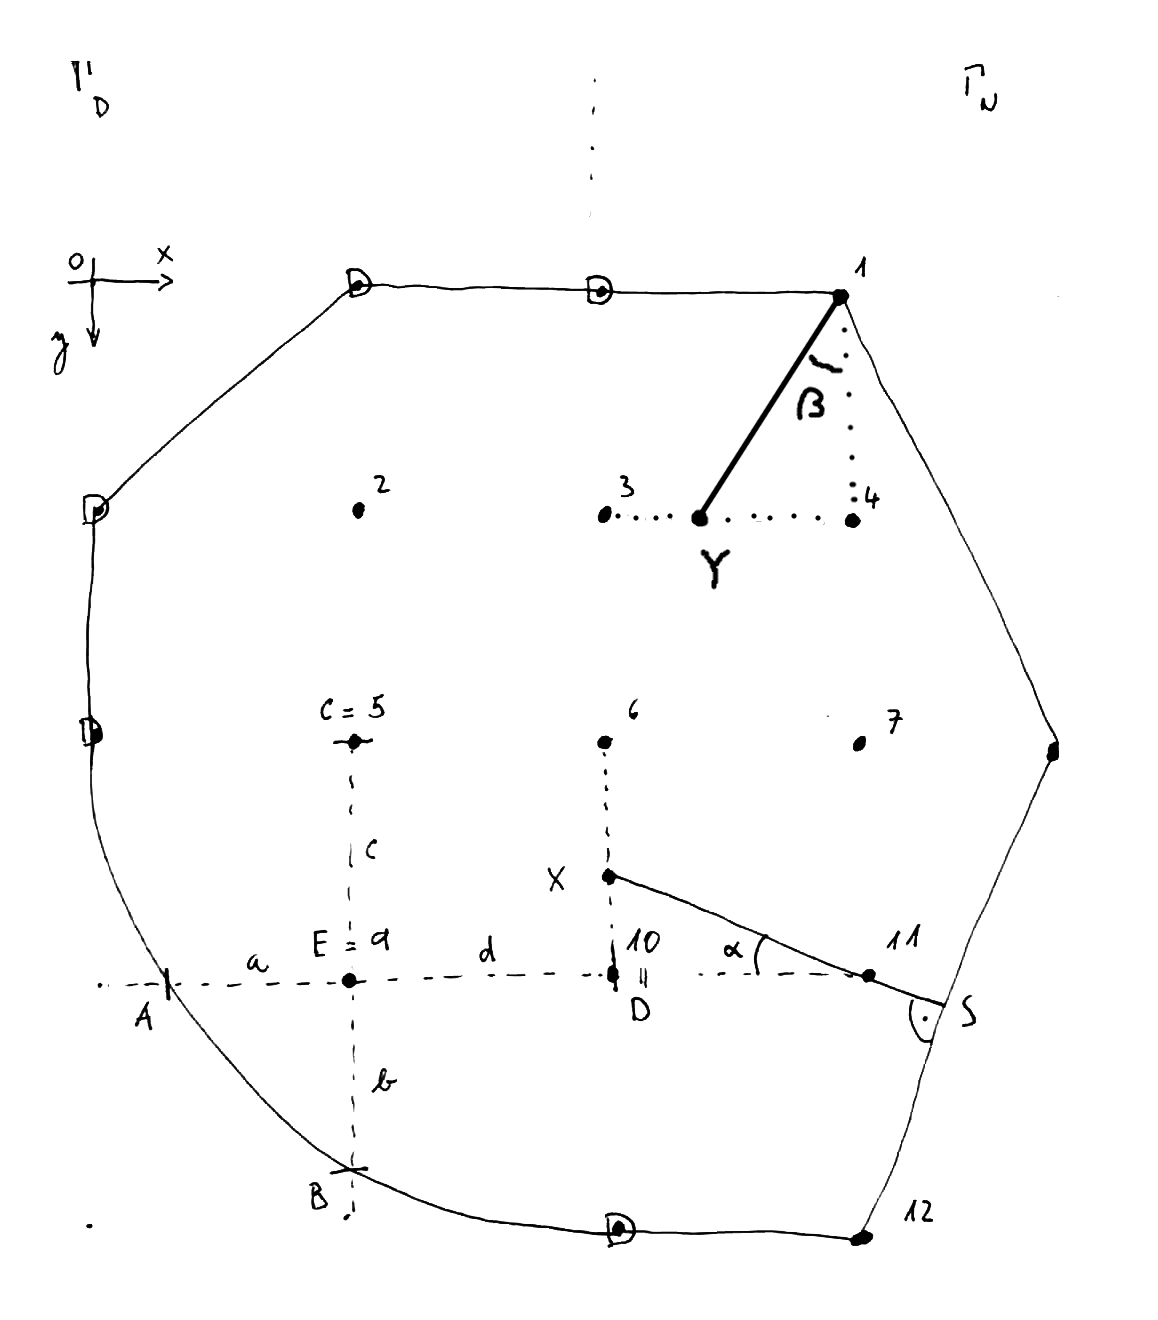
\includegraphics[width=10cm]{sit1-1.png}
  %\includegraphics[scale=0.75]{myfig.eps}
  %\includegraphics[angle=45,width=52mm]{myfig.eps}
\end{center}
\caption{Diskretizace oblasti.}
\end{figure} 

Sledujme obrázek \label{obr}, jedná se o diskretizaci oblasti $\Omega$ s krokem $h=1$. V dalším sestavíme rovnice
v bodech této sítě, pro problém s 
$p(x,y)=2x+4y$, $q(x,y)=3x-y$, $f(x,y)=y$,
Dirichletovou okrajovou podmínkou $u=\phi_D(x,y)=y$ na levé části hranice $\Gamma_D$
a Neumanovou podminkou $\frac{\prtl u}{\prtl n}=\phi_N(x,y)=5$ na pravé části $\Gamma_N$. 
Vnitřní uzly diskretizace jsou uzly číslo 6 a 7. Pro hodnotu
$u=u_6$ v bodě  $6$ dostaneme užitím \eqref{AproxL} rovnici
\[
  \big((5+8)+(3+8)+(4+10)+(4+6)+(6-2)\big)u_6-(5+8)u_7-(3+8)u_5-(4+10)u_{10}-(4+6)u_3=2.
\]
Podobně postupujeme i v bodě $7$.

Ostatní uzly nejsou vnitřní a je třeba v nich aplikovat okrajové podmínky. Nejsnazší je to v uzlech $2,3,5,10$. 
Zde hranice s Dirichletovou podmínkou prochází body sítě, takže použijeme vzorec \eqref{AproxL},
hodnoty $u$ v bodech na hranici nahradíme hodnotami $\phi_D$ a převedeme na pravou stranu. Například v bodě $2$  dostaneme rovnici
\[
  \big((3+4)+(1+4)+(2+6)+(2+2)+(3-1)\big)u_2-(3+4)u_3-(2+6)u_5=1+(1+4)1+(2+2)0.
\]

Pro aplikaci Dirichletovy podmínky v bodě $9$ můžeme použít buď interpolaci a tzv. {\it Collatzův přepis} nebo
variantu vzorce \eqref{AproxL} pro neekvidistantní síť. V prvním případě napíšeme lineární interpolaci 
funkce $u$ mezi body $A$ a $10$:
\[
  u(t)=\frac{(1+a-t)u_A+tu_{10}}{1+a}.
\]
A pro bod $9$ pak dostaneme rovnici
\[
  u_9=\frac{(1+a-a)\phi_D(A)+au_{10}}{1+a}=\frac{3}{1+a}+\frac{a}{1+a} u_{10}.
\]
Podobně bychom mohli interpolovat ve směru osy $y$ a dostat rovnici svazující hodnoty $u_9$ a $u_8$ užitím
hodnoty $\phi_D$ v bodě $B$. Nevýhodou tohoto postupu je, že není zřejmé, který směr interpolace prferovat
a dále, že takto vůbec nezachytíme rovnici \eqref{ElipRce} v bodě $9$. Nicméně lokální chyba v bodě 
$9$ je $O(h^2)$.

Druhou možností, je aproximovat rovnici v bodě $9$, resp. obecně v bodě $E$, pomocí hodnot funkce $u$
v bodech $A,B,C,D$ s obecnými vzdálenostmi $a,b,c,d$ od bodu $E$. V tomto případě má aproximace operátoru $L$ 
tvar
\begin{equation}\label{aproxLneqiv}
  L_h^*u(E)=(k_A+k_B+k_C+k_D+q(E))u(E)-k_A u(A)-k_B u(B)-k_C u(C)-k_D u(D)
\end{equation}
kde koeficienty $k_A, k_B,k_C,k_D$ mají jednotnou formu:
\[
  k_A=\frac{2}{a(a+d)}p\Big(\frac{A+E}{2}\Big),\ k_D=\frac{2}{d(a+d)}p\Big(\frac{D+E}{2}\Big)
\]
\[
  k_B=\frac{2}{b(b+c)}p\Big(\frac{B+E}{2}\Big),\ k_C=\frac{2}{c(b+c)}p\Big(\frac{C+E}{2}\Big).
\]
V našem konkrétním případě pak dostáváme v bodě $9$ rovnici
\[
    \big(k_A+k_B+k_C+k_D+(3-3)\big)u_9-k_C u_5-k_D u_{10}=3+k_A(3)+k_B(3+b)
\]
kde
\[
  k_A=\frac{2}{a(a+1)}(2-a+12),\ k_B=\frac{2}{b(b+1)}(2+12+2b),
  \ k_D=\frac{2}{1+a}(3+12),\ k_C=\frac{2}{b+1}(2+10).
\]
Tento způsob přepisu okrajové podmínky má sice lokální chybujen řádu $O(h)$, nicméně chyba vysledného přibližného řešení $u_h$ vůči přesnému řešení zůstává $O(h^2)$.

V bodech $4$ a $11$ zapíšeme Neumanovu okrajovou podmínku aproximací normálové derivace podél kolmice 
spuštěné z bodu na hranici. Pro bod $11$ dostaneme
\[
  \phi_N(S)=p(S)\frac{\prtl u}{\prtl n}\approx p(S)\frac{u_{11}-u(X)}{\frac{1}{\cos\alpha}}=
  p(S)[\cos\alpha u_{11}-(\cos\alpha-\sin\alpha)u_{10}-\sin\alpha u_{6}],
\]
kde jsme v poslední rovnosti  interpolovali hodnotu $u(X)$ mezi sousední uzly $u_{10}$ a $u_6$. Podobně dostaneme rovnici v uzlu $4$. 

V bodech $1,8,12$ není definována normála, ale přirozené je za ni vzít osu příslušných úhlů.
V případě uzlu $8$ tak dostaneme rovnici
\[
  p_8(u_8-u_7)=(4+4)(u_8-u_7)=3.
\]
Body $1$ a $12$ pak zpracujeme podobně jako body $4$ a $11$, např. pro $1$:
\[
  3=(6+0)\big(\cos\beta u_1-(\cos\beta-\sin\beta)u_4-\sin\beta u_3\big).
\]

\section{Parabolické rovnice}
Parabolické rovnice jsou zhruba řečeno eliptické rovnice doplněné o člen s časovou derivací.
Opět se omezíme na rovnice druhého řádu a to ve tvaru
\[
   \frac{\prtl u}{\prtl t}+Lu=f,
\]
kde $Lu$ je eliptický operátor. Dále budem uvažovat případ $\tn A(t,\vc x)=p(t,\vc x)\tn E$. 
 Ve dvourozměrném prostoru má takto zjednodušená rovnice tvar
\begin{multline}\label{ParEq}
 \frac{\prtl u}{\prtl t}(t,x,y)-\frac{\prtl}{\prtl x}\Big(p(t,x,y)\frac{\prtl u}{\prtl x}(t,x,y)\Big)
  -\frac{\prtl}{\prtl y}\Big(p(t,x,y)\frac{\prtl u}{\prtl y}(t,x,y)\Big)\\ 
    +q(t,x,y)u(t,x,y)=f(t,x,y).
\end{multline}
Řešení $u$ je funkcí prostorových proměnných $(x,y)$ na oblasti $\Omega$ a také funkcí času na 
nějakém daném intervalu $[0,T]$.
Jako v případě eliptických rovnic musíme zadat okrajové podmínky \eqref{BC} na $\Gamma=\prtl\Omega$ nyní ovšem
pro všechny časy. Obecně má okrajová podmínka tvar
\[
  \alpha(t,x,y)p(t,x,y)\frac{\prtl u}{\prtl n}(t,x,y)+\beta(t,x,y) u(t,x,y)=\phi(t,x,y).
\]
Rovnice \eqref{ParEq} je vzhledem k časové proměnné rovnicí prvního řádu. Podobně jako u ODR je tedy třeba zadat také počáteční podmínku
\[
   u(0,x,y)=u_0(x,y)\quad\text{ pro všechny body }(x,y)\in\Omega.
\]

\subsection{Přibližné řešení metodou sítí}
Časový člen aproximujeme jednoduchou diferencí
\[
   \frac{\prtl u}{\prtl t}(t,\vc x)\approx \frac{u(t+\tau,\vc x)-u(t,\vc x)}{\tau}.
\]
Řešení rovnice na časové hladině $t+\tau$ budeme počítat z hodnot řešení na předchozí časové hladině $t$. 
Pro aproximaci eliptického členu použijeme pro vnitřní body vzorec \eqref{AproxL}. Pokud eliptický 
člen aproximujeme na časové hladině $t$ dostáváme tzv. {\it explicitní schéma}:
\[
   \frac{u(t+\tau,\vc x)-u(t,\vc x)}{\tau} - (L_h u)(t,\vc x)= f(t,\vc x).
\]
Toto schéma má lokální chybu aproximace $O(\tau+h^2)$ a zdá se být výhodné, jelikož rovnici lze přímo použít 
k výpočtu $u(t+\tau,\vc x)$ a tím i celé nové časové hladiny. Podrobnější analýza však ukazuje, že k získání přibližného řešení, jehož chyba neroste exponenciálně s časem (takové schéma se nazývá {\it stabilní}) je třeba splnit podmínku 
\[
  \frac{\tau}{h^2}\le\text{ konstanta závislá na $p$ a $q$},
\]
což vede na velmi malý časový krok. Explicitní schéma je tedy {\it podmíněně stabilní.}
--- stabilní jen pro některé hodnoty kroků.
Další možností je aproximovat eliptický operátor na časové hladině $t+\tau$. Získáme {\it implicitní schéma}:
\[
 \frac{u(t+\tau,\vc x)-u(t,\vc x)}{\tau} - (L_h u)(t+\tau,\vc x)= f(t+\tau,\vc x).
\]
Toto schéma má opět lokální chybu $O(\tau+h^2)$ a je stabilní pro libovolný časový krok (tzv. {\it absolutně stabilní}), avšak na každé časové hladině je třeba řešit soustavu lineárních rovnic. Kombinací obou předchozích schémat je {\it Crank-Nicolsonovo schéma}:
\[
 \frac{u(t+\tau,\vc x)-u(t,\vc x)}{\tau} - \frac12\big((L_h u)(t+\tau,\vc x)+(L_h u)(t,\vc x)\big)= 
    \frac12\big(f(t+\tau,\vc x)+f(t,\vc x)\big).
\]
jeho výhodou je optimální lokální chyba $O(\tau^2+h^2)$. 

Numerické řešení si představíme, nejprve na jednorozměrném příkladě. V rovnici uvažujeme
$p=1$, $q=1$, $f=tx$. Oblastí $\Omega$ bude interval
$(0,6)$ prostorový krok sítě bude $h=2$. V bodě $x=0$ je zadána Dirichletova okrajová podmínka $u(t,0)=\phi_D(t,0)=5t+1$.
V bodě $x=6$ je zadána Neumanova podmínka $\frac{\prtl u}{\prtl x}=\phi(t,6)=-2t+1$. 
Časový krok volíme $\tau=3$. Na každé časové hladině jsou neznámé hodnoty $u$ v bodech $x=2,4,6$.
Budeme řešit vypočet vrstvy (t=10) z vrstvy (t=7). Uzly nové vrstvy označíme $21$, $22$, $23$, uzly staré vrstvy $11,12,13$
Pro vnitřní bod $22$ dostanme použitím uvedených tří schémat rovnice
\begin{align}
 &\text{explicitní:}&& \frac{u_{22}-u_{12}}{3}-\frac{2u_{12}-u_{11}-u_{13}}{4}+u_{12}=4\cdot7,\\
 &\text{implicitní:}&& \frac{u_{22}-u_{12}}{3}-\frac{2u_{22}-u_{21}-u_{23}}{4}+u_{22}=4\cdot10,\\
 &\text{C.-N.:}&& \frac{u_{22}-u_{12}}{3}-\frac{2(u_{12}+u_{22})-(u_{11}+u_{21})-(u_{13}+u_{23})}{8}
  +\frac{(u_{12}+u_{22})}{2}=2\cdot17.
\end{align}
Rovnice pro bod $21$ jsou podobné, stačí hodnoty v nultém bodě nahradit Dirichletovou podmínkou. Výsledkem jsou rovnice
\begin{align}
 &\text{explicitní:}&& \frac{u_{21}-u_{11}}{3}-\frac{2u_{11}-u_{12}}{4}+u_{11}=2\cdot7-\frac{36}{4},\\
 &\text{implicitní:}&& \frac{u_{21}-u_{11}}{3}-\frac{2u_{21}-u_{22}}{4}+u_{21}=2\cdot10-\frac{51}{4},\\
 &\text{C.-N.:}&& \frac{u_{21}-u_{11}}{3}-\frac{2(u_{11}+u_{21})-(u_{12}+u_{22})}{8}
  +\frac{(u_{11}+u_{21})}{2}=17-\frac{87}{8}.
\end{align}

V bodě $23$ potřebujem aplikovat Neumanovu podmínku. Ukažme nejprve jak se postupuje v obecném případě. V bodě $x$ máme dánu Neumanovu podmínku s normálou v kladném směru (bod na pravém okraji oblasti)
\[
  p(x)\frac{\prtl u}{\prtl x}(x)=\phi_N(x).
\]
Rovnici v bodě $x$ aproximujeme podobně jako ve vnitřních bodech, ale pro hlavní část eliptického členu použijeme následující přepis 
\[
 \frac{\prtl}{\prtl x}\Big( p(x)\frac{\prtl u}{\prtl x}(x)\Big)\approx 
    \frac{\big(p\frac{\prtl u}{\prtl x}\big)(x)-\big(p\frac{\prtl u}{\prtl x}\big)(x-\frac{h}2)}{\frac{h}{2}}
\approx
   \frac{2\phi_N(x)}{h}-\frac{2p(x-\frac{h}2)}{h}\frac{u(x)-u(x-h)}{h}.
\]
V případě normály v záporném směru (bod na levém kraji) dostaneme:
\[
 \frac{\prtl}{\prtl x}\Big( p(x)\frac{\prtl u}{\prtl x}(x)\Big)\approx 
   \frac{2\phi_N(x)}{h}+\frac{2p(x+\frac{h}2)}{h}\frac{u(x+h)-u(x)}{h}.
\]
Rovnice pro bod $23$ tedy vyjdou
\begin{align}
 &\text{explicitní:}&& \frac{u_{23}-u_{13}}{3}+\frac{u_{13}-u_{12}}{2}+u_{13}=6\cdot7-\frac{13}{2},\\
 &\text{implicitní:}&& \frac{u_{23}-u_{13}}{3}+\frac{u_{23}-u_{22}}{2}+u_{23}=6\cdot10-\frac{19}{2},\\
 &\text{C.-N.:}&& \frac{u_{23}-u_{13}}{3}+\frac{(u_{13}+u_{23})-(u_{12}+u_{22})}{4}
  +\frac{(u_{13}+u_{23})}{2}=3\cdot17-8.
\end{align}

\subsection{Další příklady}
{\bf 1D, obecný případ} Budeme řešit rovnici \eqref{ParEq} pro $p=2x+t$, $q=xt$, $f=x-t$ na $\Omega=[0,6]$ s prostorovým
krokem $h=3$. V bodě $x=0$ je dána Neumanova podmínka $\phi_N=20-t^2$, v bodě $6$ je dána Dirichletova podmínka
$\phi_D=1-t$. Časový krok $\tau=2$. Napište rovnice pro výpočet časové hladiny $t=6$ (uzly $20$ a $21$
z časové hladiny $t=4$ (uzly $10$ a $11$) pro explicitní a implicitní schéma.

explicitní:
\[
   \frac{u_{21}-u_{11}}{2}-\frac{20u_{11}-7u_{10}}{9}+12u_{11}=-1+\frac{3\cdot13}{9}
\]
\[
   \frac{u_{20}-u_{10}}{2}-\frac{14(u_{11}-u_{10})}{9}+0u_{10}=-4+\frac{2\cdot4}{3}
\]

implicitní:
\[
   \frac{u_{21}-u_{11}}{2}-\frac{24u_{21}-9u_{20}}{9}+18u_{11}=-3+\frac{5\cdot15}{9}
\]
\[
   \frac{u_{20}-u_{10}}{2}-\frac{18(u_{21}-u_{20})}{9}+0u_{20}=-6-\frac{2\cdot16}{3}
\]


{\bf 2D, obdelník} Řešme rovnici
\[
 \frac{\prtl u}{\prtl t} -\frac{\prtl^2 u}{\prtl x^2}-3\frac{\prtl^2 u}{\prtl y^2}=3x-2y+t
\]
na oblasti $\Omega=[0,\frac{10}{2}]\times[0,\frac{14}{3}]$ s prostorovým krokem $h=2$ a Dirichletovou okrajovou
podmínkou $\phi_D=3x+t+y$ na celé hranici. Časový krok $\tau=1$. Body $(2,2)$, $(4,2)$, $(2,4)$, $(4,4)$ 
na časové hladině $t=5$ označíme $21$, $22$, $23$, $24$. Stejné body v čase $t=4$ označíme 
$11$, $12$, $13$, $14$. Napište rovnice pro výpočet časové hladiny $t=5$ pro explicitní a implicitní schéma. 
V bodě $23$ použijte Collatzovu interpolaci, v bodech $22$, $24$ vzorec \eqref{aproxLneqiv}.

Explicitní:
\[
  \frac{u_{21}-u_{11}}{1}-\frac{2u_{11}+6u_{11}-u_{12}-3u_{13}}{4}=6-4+4-\tfrac64-\tfrac{30}{4}  
\]
\[
  \frac{u_{22}-u_{12}}{1}-(\tfrac26+\tfrac23)u_{12}+\tfrac26u_{11}-\tfrac64u_{12}+\tfrac34u_{14}
   =12-4+4-\tfrac23(15+4+2)-\tfrac{3}{4}(12+4+0)  
\]
\[
  \frac{\frac23u_{21}-2\cdot(6+5+\frac{14}{3})}{\frac83}=u_{23}  
\]
\[
  \frac{u_{24}-u_{14}}{1}-(\tfrac26+\tfrac23)u_{14}+\tfrac26u_{13}-(\tfrac38+\tfrac98)u_{14}+\tfrac38u_{12}
   =12-8+4-\tfrac23(15+4+4)-\tfrac98(12+4+\tfrac{14}{3})  
\]

Implicitní:
\[
  \frac{u_{21}-u_{11}}{1}-\frac{2u_{21}+6u_{21}-u_{22}-3u_{23}}{4}=6-4+5-\tfrac{7}{4}-\tfrac{33}{4}  
\]
\[
  \frac{u_{22}-u_{12}}{1}-(\tfrac26+\tfrac23)u_{22}+\tfrac26u_{21}-\tfrac64u_{22}+\tfrac34u_{24}
   =12-4+5-\tfrac23(15+5+2)-\tfrac34(12+5+0)  
\]
\[
  \frac{\frac23u_{21}-2\cdot(6+5+\frac{14}{3})}{\frac83}=u_{23}  
\]
\[
  \frac{u_{24}-u_{14}}{1}-(\tfrac26+\tfrac23)u_{24}+\tfrac26u_{23}-(\tfrac38+\tfrac98)u_{24}+\tfrac38u_{22}
   =12-8+5-\tfrac23(15+5+4)-\tfrac98(12+5+\tfrac{14}{3})  
\]

Pro implicitní schéma napište soustavu rovnic pro výpočet časové vrstvy $t=5$ pokud je $u$ v čase $t=4$ rovno konstantě $1$. 
\[
  -u_{21}+\frac14u_{22}+\frac34u_{23}=-2
\]
\[
  -\frac32u_{22}+\frac13u_{2}+\frac34u_{24}=-\frac{161}{12}
\]
\[
 \frac14u_{21}-u_{23}=\frac{47}{12}
\]
\[
 -\frac32u_{24}+\frac13u_{23}+\frac38u_{22}=-\frac{243}{8}
\]

\begin{thebibliography}{9}
\bibitem{Vitasek}
	Emil Vitásek : {\it Numerické metody.}
	SNTL Praha, 1987. Je v knihovně.
\end{thebibliography}
\end{document}
